% !TEX root = 00_arbeit.tex

%---------------------------------------------------------------------------------
%% Titelseite
\begin{titlepage}
\thispagestyle{empty}
\begin{doublespace}
\centering

%\Mygrid

\begin{center}
	
\includegraphics[width=1.0\textwidth]{Bilder/Offiziell/TUBSIF.pdf}
\end{center}

\vspace{1cm}

\begin{singlespacing}
    {\small Masterarbeit\\zur Erlangung des akademischen Grades\\Master of Science\\ \vspace{2cm}}
\end{singlespacing}


{\huge \textcolor{red}{\textbf{\titel}}}\\ \vspace{2cm}
{\small Vorgelegt von:\\ \vspace{1cm}}

{\Large B.Sc. \name}\\

\begin{singlespacing}
    albrecht.dennis@live.de\\Wirtschaftsingenieurwesen Elektrotechnik\\Matr.-Nr.: 4603931\\
\end{singlespacing}

\vspace{6cm}


%\abgabedatum\\ \vspace{2cm}
\begin{singlespacing}
    Carl-Friedrich-Gauß Fakultät: Institut für Finanzwirtschaft\\Technische Universität Braunschweig\\Braunschweig, März 2018\\
\end{singlespacing}

\begin{textblock*}{20mm}(25mm,195mm)
\raggedright
    Betreuer:
\end{textblock*}

\begin{textblock*}{80mm}(25mm,200mm)
\raggedright
    Dipl.-Wirtsch.-Ing. Thomas Paulsen
\end{textblock*}



\begin{textblock*}{38mm}(25mm,218mm)
\raggedright
    Erstprüfer:
\end{textblock*}

\begin{textblock*}{38mm}(25mm,223mm)
\raggedright
    Prof. Dr. Marc Gürtler
\end{textblock*}



\begin{textblock*}{48mm}(137mm,218mm)
\raggedright
    Zweitprüfer:
\end{textblock*}

\begin{textblock*}{48mm}(137mm,223mm)
\raggedright
    Prof. Dr. Christian Leßmann
\end{textblock*}


\end{doublespace}
\end{titlepage}
%---------------------------------------------------------------------------------
\blankpage
%---------------------------------------------------------------------------------
%% Aufgabenstellung

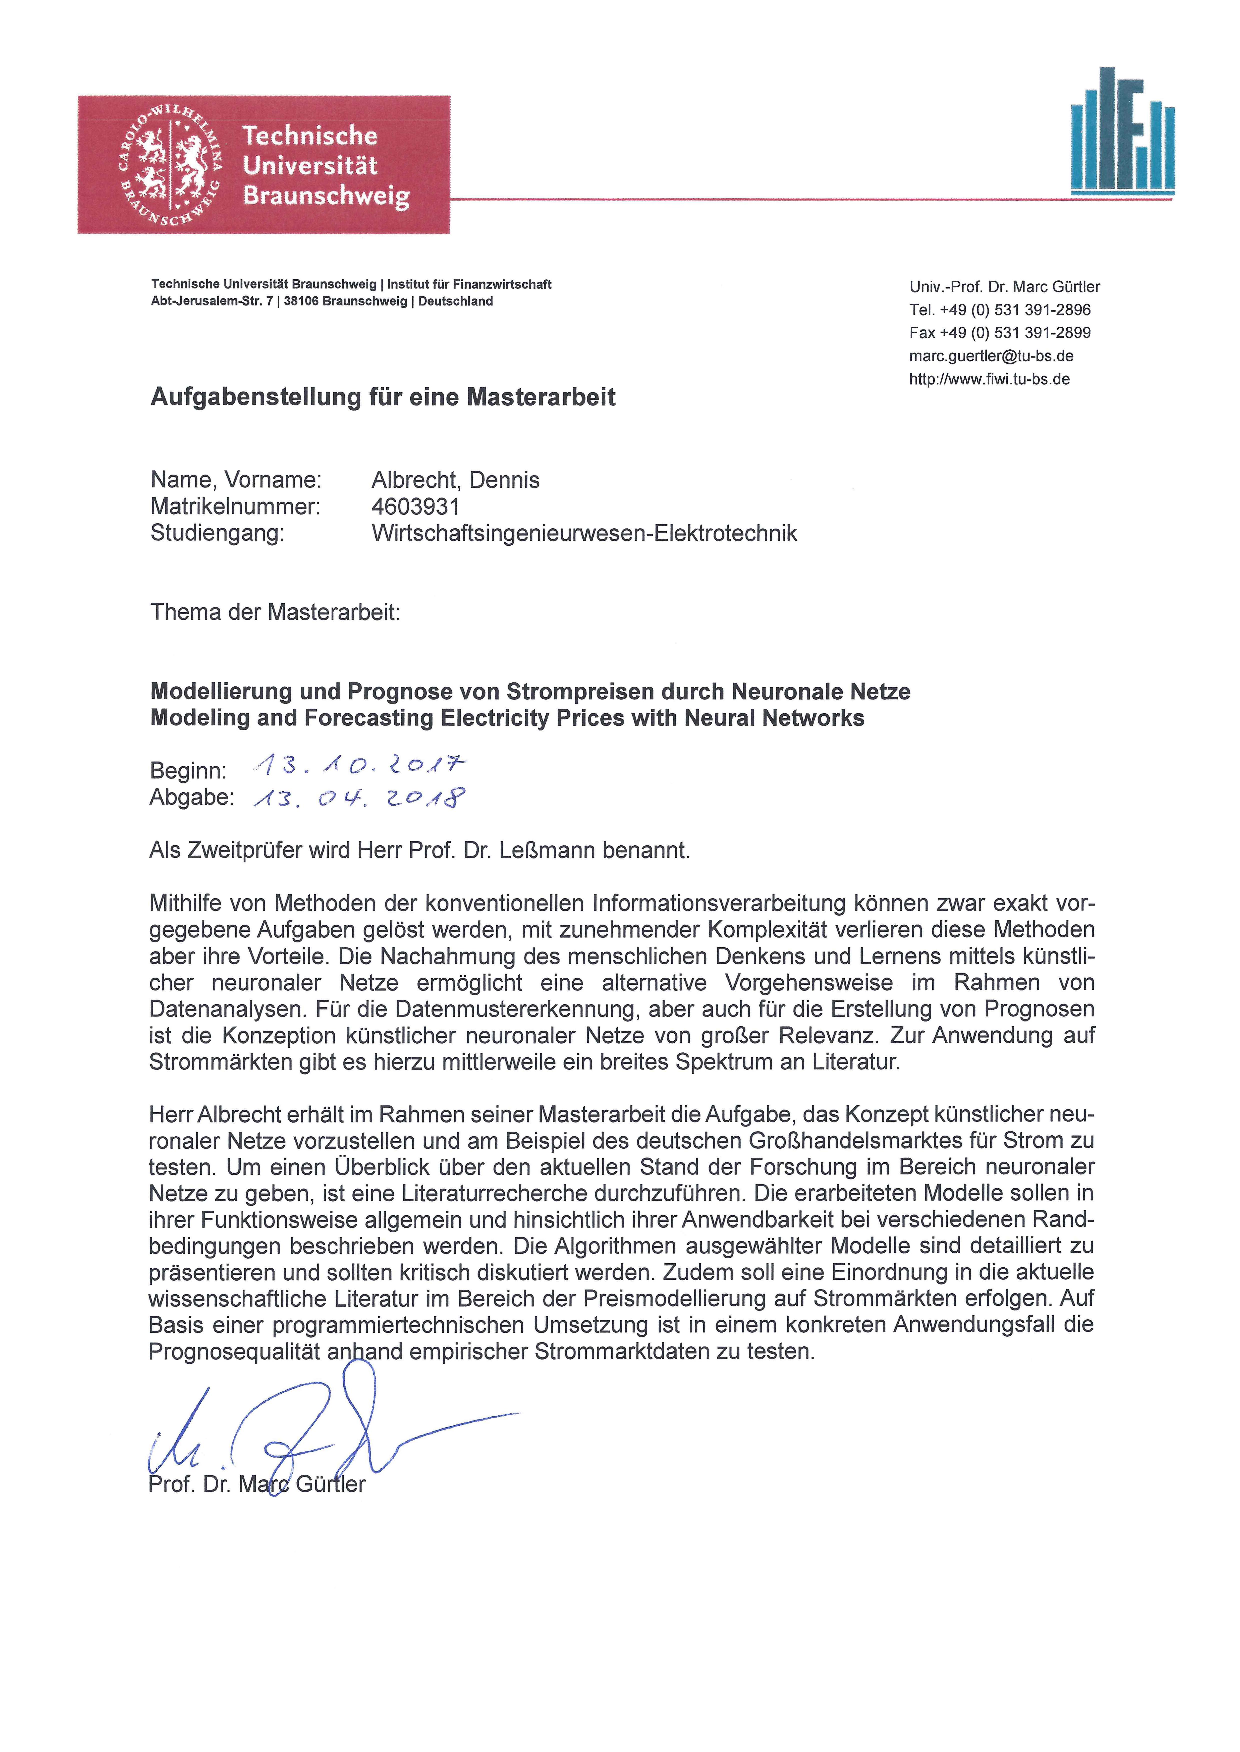
\includepdf[pages=-]{Bilder/Offiziell/Aufgabenstellung_Masterarbeit_600dpi_rot.pdf}    % Fügt alle Seiten des PDF Dokumentes ein

%---------------------------------------------------------------------------------
\newpage
%---------------------------------------------------------------------------------
%% Eidesstattliche Erklärung

%\thispagestyle{empty}
\pagenumbering{Roman}
\setcounter{page}{4}

{\LARGE \textbf{Eidesstattliche Erklärung}}\\ \vspace{1cm}

Ich erkläre hiermit an Eides statt, dass ich die vorliegende  Masterarbeit „\titel“ selbstständig verfasst sowie alle benutzten Quellen und Hilfsmittel vollständig angegeben habe.\\ \vspace{1cm}

Braunschweig, den \abgabedatum\\ \vspace{1cm}

\name
%---------------------------------------------------------------------------------